
\frame{\frametitle{Legasthenie}
	\begin{itemize}
 		\item Eine Störung der auditiven und visuellen Wahrnehmungsverarbeitung, die zu einer Lese- und Rechtschreibschwäche führt, trotz normal entwickelter Intelligenz. \pause
 		\item erblich bedingt \pause
 		\item taucht häufig gemeinsam mit AD(H)S auf\pause
 		\item umstritten ob heilbar oder nicht
 	\end{itemize}
 }

\frame{\frametitle{Legasthenie}

 	\begin{figure}[t]
	\centering
		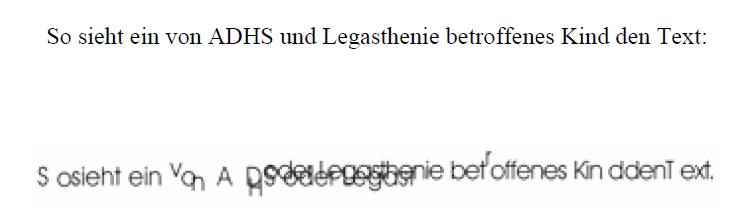
\includegraphics[width=1.0\textwidth]{Slides/Gruende/Daten/legastheneWahrnehmung.PNG}
	\end{figure}
 }